%%%%%%%%%%%%%%%%%%%%%%%%%%%%%%%%%%%%%%%%%
% Lachaise Assignment
% LaTeX Template
% Version 1.0 (26/6/2018)
%
% This template originates from:
% http://www.LaTeXTemplates.com
%
% Authors:
% Marion Lachaise & François Févotte
% Vel (vel@LaTeXTemplates.com)
%
% License:
% CC BY-NC-SA 3.0 (http://creativecommons.org/licenses/by-nc-sa/3.0/)
% 
%%%%%%%%%%%%%%%%%%%%%%%%%%%%%%%%%%%%%%%%%

%----------------------------------------------------------------------------------------
%	PACKAGES AND OTHER DOCUMENT CONFIGURATIONS
%----------------------------------------------------------------------------------------

\documentclass{article}

%%%%%%%%%%%%%%%%%%%%%%%%%%%%%%%%%%%%%%%%%
% Lachaise Assignment
% Structure Specification File
% Version 1.0 (26/6/2018)
%
% This template originates from:
% http://www.LaTeXTemplates.com
%
% Authors:
% Marion Lachaise & François Févotte
% Vel (vel@LaTeXTemplates.com)
%
% License:
% CC BY-NC-SA 3.0 (http://creativecommons.org/licenses/by-nc-sa/3.0/)
% 
%%%%%%%%%%%%%%%%%%%%%%%%%%%%%%%%%%%%%%%%%

%----------------------------------------------------------------------------------------
%	PACKAGES AND OTHER DOCUMENT CONFIGURATIONS
%----------------------------------------------------------------------------------------

\usepackage{keystroke} % https://ctan.crest.fr/tex-archive/macros/latex/contrib/keystroke/key-test.pdf

\usepackage{amsmath,amsfonts,stmaryrd,amssymb} % Math packages

\usepackage{minted} 

\usepackage{enumerate} % Custom item numbers for enumerations

\usepackage[ruled]{algorithm2e} % Algorithms

\usepackage[framemethod=tikz]{mdframed} % Allows defining custom boxed/framed environments

\usepackage{listings} % File listings, with syntax highlighting
\lstset{
	basicstyle=\ttfamily, % Typeset listings in monospace font
}

\usepackage{dirtree}

\usepackage{hyperref}

\usepackage{xcolor}

\usepackage{graphicx}

%----------------------------------------------------------------------------------------
%	DOCUMENT MARGINS
%----------------------------------------------------------------------------------------

\usepackage{geometry} % Required for adjusting page dimensions and margins

\geometry{
	paper=a4paper, % Paper size, change to letterpaper for US letter size
	top=2.5cm, % Top margin
	bottom=3cm, % Bottom margin
	left=2.5cm, % Left margin
	right=2.5cm, % Right margin
	headheight=14pt, % Header height
	footskip=1.5cm, % Space from the bottom margin to the baseline of the footer
	headsep=1.2cm, % Space from the top margin to the baseline of the header
	%showframe, % Uncomment to show how the type block is set on the page
}

%----------------------------------------------------------------------------------------
%	FONTS
%----------------------------------------------------------------------------------------

\usepackage[utf8]{inputenc} % Required for inputting international characters
\usepackage[T1]{fontenc} % Output font encoding for international characters

\usepackage{XCharter} % Use the XCharter fonts

%----------------------------------------------------------------------------------------
%	COMMAND LINE ENVIRONMENT
%----------------------------------------------------------------------------------------

% Usage:
% \begin{commandline}
%	\begin{verbatim}
%		$ ls
%		
%		Applications	Desktop	...
%	\end{verbatim}
% \end{commandline}

\mdfdefinestyle{commandline}{
	leftmargin=10pt,
	rightmargin=10pt,
	innerleftmargin=15pt,
	middlelinecolor=black!50!white,
	middlelinewidth=2pt,
	frametitlerule=false,
	backgroundcolor=black!5!white,
	frametitle={Command Line},
	frametitlefont={\normalfont\sffamily\color{white}\hspace{-1em}},
	frametitlebackgroundcolor=black!50!white,
	nobreak,
}

% Define a custom environment for command-line snapshots
\newenvironment{commandline}{
	\medskip
	\begin{mdframed}[style=commandline]
}{
	\end{mdframed}
	\medskip
}

%----------------------------------------------------------------------------------------
%	FILE CONTENTS ENVIRONMENT
%----------------------------------------------------------------------------------------

% Usage:
% \begin{file}[optional filename, defaults to "File"]
%	File contents, for example, with a listings environment
% \end{file}

\mdfdefinestyle{file}{
	innertopmargin=1.6\baselineskip,
	innerbottommargin=0.8\baselineskip,
	topline=false, bottomline=false,
	leftline=false, rightline=false,
	leftmargin=2cm,
	rightmargin=2cm,
	singleextra={%
		\draw[fill=black!10!white](P)++(0,-1.2em)rectangle(P-|O);
		\node[anchor=north west]
		at(P-|O){\ttfamily\mdfilename};
		%
		\def\l{3em}
		\draw(O-|P)++(-\l,0)--++(\l,\l)--(P)--(P-|O)--(O)--cycle;
		\draw(O-|P)++(-\l,0)--++(0,\l)--++(\l,0);
	},
	nobreak,
}

% Define a custom environment for file contents
\newenvironment{file}[1][File]{ % Set the default filename to "File"
	\medskip
	\newcommand{\mdfilename}{#1}
	\begin{mdframed}[style=file]
}{
	\end{mdframed}
	\medskip
}

%----------------------------------------------------------------------------------------
%	NUMBERED QUESTIONS ENVIRONMENT
%----------------------------------------------------------------------------------------

% Usage:
% \begin{question}[optional title]
%	Question contents
% \end{question}

\mdfdefinestyle{question}{
	innertopmargin=1.2\baselineskip,
	innerbottommargin=0.8\baselineskip,
	roundcorner=5pt,
	nobreak,
	singleextra={%
		\draw(P-|O)node[xshift=1em,anchor=west,fill=white,draw,rounded corners=5pt]{%
		Question \theQuestion\questionTitle};
	},
}

\newcounter{Question} % Stores the current question number that gets iterated with each new question

% Define a custom environment for numbered questions
\newenvironment{question}[1][\unskip]{
	\bigskip
	\stepcounter{Question}
	\newcommand{\questionTitle}{~#1}
	\begin{mdframed}[style=question]
}{
	\end{mdframed}
	\medskip
}

%----------------------------------------------------------------------------------------
%	WARNING TEXT ENVIRONMENT
%----------------------------------------------------------------------------------------

% Usage:
% \begin{warn}[optional title, defaults to "Warning:"]
%	Contents
% \end{warn}

\mdfdefinestyle{warning}{
	topline=false, bottomline=false,
	leftline=false, rightline=false,
	nobreak,
	singleextra={%
		\draw(P-|O)++(-0.5em,0)node(tmp1){};
		\draw(P-|O)++(0.5em,0)node(tmp2){};
		\fill[black,rotate around={45:(P-|O)}](tmp1)rectangle(tmp2);
		\node at(P-|O){\color{white}\scriptsize\bf !};
		\draw[very thick](P-|O)++(0,-1em)--(O);%--(O-|P);
	}
}

% Define a custom environment for warning text
\newenvironment{warn}[1][Warning:]{ % Set the default warning to "Warning:"
	\medskip
	\begin{mdframed}[style=warning]
		\noindent{\textbf{#1}}
}{
	\end{mdframed}
}

%----------------------------------------------------------------------------------------
%	INFORMATION ENVIRONMENT
%----------------------------------------------------------------------------------------

% Usage:
% \begin{info}[optional title, defaults to "Info:"]
% 	contents
% 	\end{info}

\mdfdefinestyle{info}{%
	topline=false, bottomline=false,
	leftline=false, rightline=false,
	nobreak,
	singleextra={%
		\fill[black](P-|O)circle[radius=0.4em];
		\node at(P-|O){\color{white}\scriptsize\bf i};
		\draw[very thick](P-|O)++(0,-0.8em)--(O);%--(O-|P);
	}
}

% Define a custom environment for information
\newenvironment{info}[1][Info:]{ % Set the default title to "Info:"
	\medskip
	\begin{mdframed}[style=info]
		\noindent{\textbf{#1}}
}{
	\end{mdframed}
}
 % Include the file specifying the document structure and custom commands

%----------------------------------------------------------------------------------------
%	ASSIGNMENT INFORMATION
%----------------------------------------------------------------------------------------

\title{Synthèse d'image : compte rendu} % Title of the assignment

\author{Valentin VERSTRACTE \& Evan PETIT}

\date{L3 --- \today} % University, school and/or department name(s) and a date

%----------------------------------------------------------------------------------------

\begin{document}

\maketitle % Print the title

%----------------------------------------------------------------------------------------
%	INTRODUCTION
%----------------------------------------------------------------------------------------

\section*{Introduction} % Unnumbered section

%----------------------------------------------------------------------------------------
%	Répertoire
%----------------------------------------------------------------------------------------

\section{Une conception orienté objet} % Numbered section

Chaque primitive, courbe de bézier et courbe paramétrique sont représenter par des classes. Chacune d'elle est dérivée de la classe objet. Cette classe objet permet de contenir et d'effectuer la translation, la rotation, les couleurs et si "l'objet" est lié à une texture ou non. Pour appliquer tout cela, il suffit d'appeler this->onDraw() qui s'occupe de tout le reste. Ensuite, dans ces classes dérivée, le constructeur initialise les différents attributs. Il appel la fonction draw qui, comme l'indique son nom, dessine. Cette structure aussi efficace que pratique exige cependant des conditions : La méthode draw doit commencer par un glPushMatrix() et this->onDraw() (hérité de objet) et doit finir par un glPopMatrix(). 

\begin{figure}[!htb]
	\begin{minipage}{0.5\textwidth}
    	\centering
    	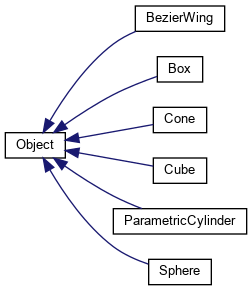
\includegraphics[height=6cm]{./assets/class_hierarchy.png}
    	\caption{Diagramme de classes}
    	\label{fig:class_hierarchy}
	\end{minipage}
	\hfill
	\begin{minipage}{0.5\textwidth}
    	\centering
    	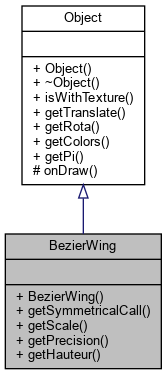
\includegraphics[height=6cm]{./assets/class_hierarchy_bezier.png}
    	\caption{Exemple diagramme classe bézier}
    	\label{fig:class_hierarchy_bezier}
	\end{minipage}
\end{figure}


\subsection{Le cylindre paramétrique}

\begin{figure}[!htb]
	\begin{minipage}{0.5\textwidth}
    	\centering
    	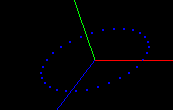
\includegraphics[height=4.5cm]{./assets/cylindre_para_0.png}
		\caption{30 points évalués}
    	\label{fig:cylindre_para_0}
	\end{minipage}
	\hfill
	\begin{minipage}{0.5\textwidth}
    	\centering
    	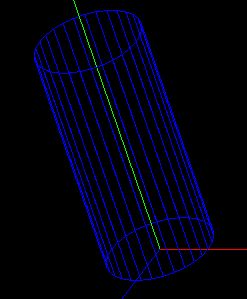
\includegraphics[height=6cm]{./assets/cylindre_para_1.png}
    	\caption{La construction des polygones}
    	\label{fig:cylindre_para_1}
	\end{minipage}
\end{figure}

Le cylindre paramétrique dépend de 3 paramètres importants : le rayon, la hauteur et la précision. Le rayon et la hauteur sont plutôt révélateur de ce qu'ils sont. Cependant comme on utilise une équation paramétrique il est nécessaire d'évaluer les points à un instant t. La précision représente justement le nombre d'évaluation que l'on va effectuer. Elle représente aussi le nombre de face que le cylindre va obtenir. 
\newline
\newline
Ainsi pour construire ce cylindre plusieurs étapes sont importantes :

\begin{itemize}
\item On évalue les points autour d'un cercle de rayon donner en paramètre. On obtient pour chaque point une coordonnée (x,z) que l'on stock dans un tableau à l'indice t. Exemple de 30 points figure \ref{fig:cylindre_para_0}
\item On crée des polygones à partir de ces points :
	\begin{itemize}
		\item La partie inférieur gauche est égale à x(t),0,z(t)
		\item La partie inférieur droite est égale à x(t+1),0,z(t+1)
		\item La partie supérieur gauche est égale à x(t),hauteur,z(t)
		\item La partie supérieur droite est égale à x(t+1),0,z(t+1)
	\end{itemize}
Exemple de polygones avec les 30 points précédent (vision fil de fer) figure \ref{fig:cylindre_para_1}
\item On ferme la partie inférieur et supérieur en créent 2 polygones en utilisant tout les points contenu dans t. On le fait d'abord pour un premier polygone à la hauteur 0, puis pour le deuxième à la hauteur donnée en paramètre
\end{itemize}


\subsection{Les ailes, deux courbes de bézier}

\subsubsection{La représentation 2D}

Les ailes sont construites à partir de deux courbes de bézier cubiques. Une courbe de bézier cubique est une courbe polynomiale paramétrique à partir de 4 points de contrôle. On rappel l'équation pour évaluer un point d'une courbe de bézier :
\equabezier
Où P0, P1, P2, P3 représente les points de contrôle. Ainsi tout comme notre cylindre paramétrique, cette classe aura besoin d'un paramètre précision pour déterminer le nombre de points à évaluer.

\begin{figure}[!htb]
	\begin{minipage}{0.5\textwidth}
    	\centering
    	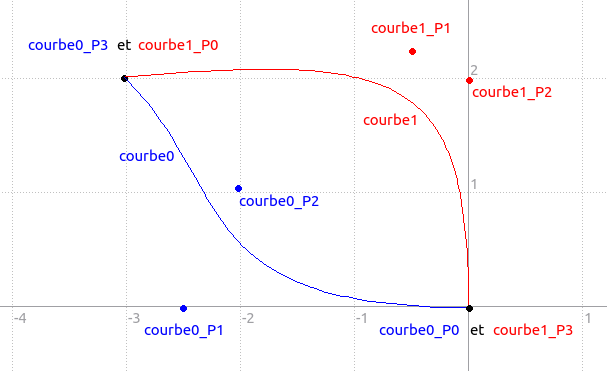
\includegraphics[height=4.5cm]{./assets/kig_bezier.png}
    	\caption{Courbes de bézier sur kig}
    	\label{fig:kig_bezier}
	\end{minipage}
	\hfill
	\begin{minipage}{0.5\textwidth}
    	\centering
    	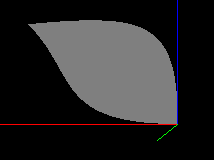
\includegraphics[height=4.5cm]{./assets/2D_bezier.png}
    	\caption{Courbes de bézier 2D openGL}
    	\label{fig:2D_bezier}
	\end{minipage}
\end{figure}

La figure 2 montre la représentation 2D et le choix des différents points de contrôle pour les deux courbes. Pour représenter cette aile avec openGL, on va construire un polygone en 2D où chaque point du polygone appartient à une de nos deux courbes de bézier. On commence par les points de la courbe en bleu puis on finit avec les points de celle en rouge. On commence de (0,0), on monte jusqu'en (-3,2) et on redescend jusqu'en (0,0). On obtient une aile en 2D cf figure \ref{fig:2D_bezier}. 
\newline
\newline
Pour simplifier les dimensions deux opérations supplémentaires sont effectuer au tout début. Les points de contrôle on un maximum de 3 en x et z. On divise d'abord tout les points de contrôle par 3 pour que la taille maximum de l'aile soit de 1 en x et z. Ensuite, on ne souhaite pas forcément que les ailes soit aussi petite. On rajoute un paramètre dimension dans notre classe et on multiplie tout nos points de contrôle par ce paramètre. Ainsi la taille maximum en x et z serra la valeur de "dimension".

\subsubsection{La représentation 3D}

\begin{figure}[!htb]
	\centering
	\begin{minipage}{0.3\textwidth}
    	\centering
    	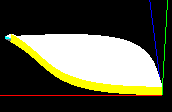
\includegraphics[height=3cm]{./assets/3D_0_bezier.png}
    	\caption{Vue 3D 0}
    	\label{fig:3D_0_bezier}
	\end{minipage}
	\begin{minipage}{0.3\textwidth}
    	\centering
    	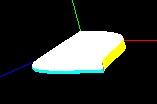
\includegraphics[height=3cm]{./assets/3D_1_bezier.png}
    	\caption{Vue 3D 1}
    	\label{fig:3D_1_bezier}
	\end{minipage}
	\begin{minipage}{0.3\textwidth}
    	\centering
    	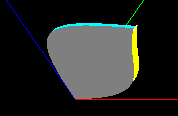
\includegraphics[height=3cm]{./assets/3D_2_bezier.png}
    	\caption{Vue 3D 2}
    	\label{fig:3D_2_bezier}
	\end{minipage}
\end{figure}
En gris, la même aile et "premier polygone" que la figure \ref{fig:2D_bezier}. En blanc "deuxième polygone". En bleu "troisième polygone". En jaune "quatrième polygone"
\newline
\newline
La représentation 3D est constituer de 4 polygones. Les deux premiers sont deux ailes 2D de hauteur 0 et une deuxième de hauteur de 0.4 dans le plus grand des cas. La deuxième est légèrement "penché". Sa hauteur vers la courbe bleue (cf figure \ref{fig:kig_bezier}) commence vers 1/3 de la hauteur max tandis que vers la courbe rouge, elle est de 0.4 (hauteur max). Le troisième est constituer des points de la courbe bleu de la figure \ref{fig:kig_bezier} en bleue qui commence à la hauteur de la première aile 2D jusqu'à la hauteur de la deuxième aile 2D. La quatrième est équivalente hormis qu'on l'applique pour la courbe rouge de figure \ref{fig:kig_bezier}.

\subsubsection{Le problème de symétrie}

\begin{figure}[!htb]
	\centering
	\begin{minipage}{0.3\textwidth}
    	\centering
    	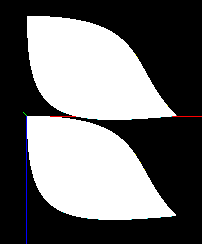
\includegraphics[height=4cm]{./assets/3D_symetrie_0_bezier.png}
    	\caption{Symétrie incorrecte}
    	\label{fig:3D_symetrie_0_bezier}
	\end{minipage}
	\begin{minipage}{0.3\textwidth}
    	\centering
    	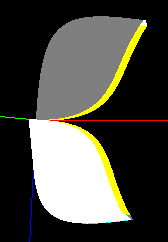
\includegraphics[height=4cm]{./assets/3D_symetrie_1_bezier.png}
    	\caption{Tentative de rotation}
    	\label{fig:3D_symetrie_1_bezier}
	\end{minipage}
	\begin{minipage}{0.3\textwidth}
    	\centering
    	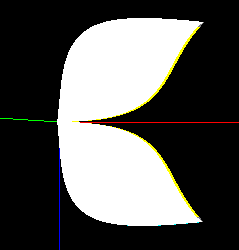
\includegraphics[height=4cm]{./assets/3D_symetrie_2_bezier.png}
    	\caption{Problème résolu}
    	\label{fig:3D_symetrie_2_bezier}
	\end{minipage}
\end{figure}

Un problème inattendu pour essayer de créer des ailes comme dans la figure \ref{fig:3D_symetrie_2_bezier} (résultat final) a été tout d'abord celui de la figure \ref{fig:3D_symetrie_0_bezier}. Une rotation a été naïvement tenté pour résoudre le problème cf figure 9 mais le résultat n'est toujours pas bon (notamment à cause de la hauteur de 1/3 (cf figure \ref{fig:3D_1_bezier} le bleu) "en dessous au lieu de haut dessus"). Pour obtenir la figure \ref{fig:3D_symetrie_2_bezier} et résoudre le problème il a été décidé de jouer avec les coordonnées des points de contrôle. Il suffit de prendre l'opposé en z pour obtenir une deuxième aile symétrique. Ainsi un booléen symetricall a été rajouté à notre classe pour préciser si on souhaite prendre des points de coordonnées avec l'opposé en z. 

\subsection{La box}

\subsection{Les primitives}

%------------------------------------------------

\section{Les textures}

Une texture est représenté par une classe. Son constructeur prend en paramètre un string qui s'occupe de charger en mémoire la texture. Ensuite, pour décrire qu'il faut utiliser cette texture il suffit d'appeler enableTexture() sur l'objet instancié. Cette fonction appelle simplement glTextImage2D() de glut avec les paramètres nécessaire.  

%------------------------------------------------

\section{Les animations}

\subsection{Une animation automatique}

L'animation automatique se porte les ailes du dragon. On incrémente un angle de + ou - 25 ° se qui donne au dragon l'impression de voler. La logique algorithmique est plutôt simple. On incrémente un tout petit l'angle dans la fonction anim ( appeler par glut chaque fois qu'il ne fait rien ). Si l'angle est supérieur à 25 on décremente. Si l'angle est inférieur à -25 on incrémente. 
 
\subsection{Une animation manuelle}

L'animation n'est pas très impressionnante. En peut juste baisser ou lever la queue en fonction des touches h et n

%------------------------------------------------

\section{Les touches disponibles}

\begin{itemize}
\item \keystroke{p} : affichage du carré plein
\item \keystroke{f} : affichage du mode de fil de fer
\item \keystroke{s} : affichage en mode de sommets seuls
\item \keystroke{z} : permet de zoomer
\item \keystroke{Z} : permet de dézoomer 
\item \keystroke{h} : élève la queue du dragon
\item \keystroke{n} : abaisse la queue du dragon 
\item \keystroke{q} : quitter l'application 
\item \UArrow \DArrow \LArrow \RArrow : déplace la caméra en haut, en bas, à droite, à gauche
\end{itemize}

%----------------------------------------------------------------------------------------

\end{document}
